Cleaving and polishing add a systematic dispersion $\sigma_{sys-SF}$ to the instrinsic fiber response. In addition, the position of the connectors that lock the fiber to the experimental setup of Figure \ref{fig:SetUpFiberCharacterization} produces an additional systematic uncertainty $\sigma_{sys-pos}$. Since both uncertainties are independent, the total systematic uncertainty is given by,

\begin{equation}
\sigma_{sys} = \sqrt{\sigma^2_{sys-SF} + \sigma^2_{sys-pos} }
\label{eq:TotalUncertaintyFiberCharacterization}
\end{equation}
The uncertainty due to fiber positioning $\sigma_{sys-pos}$ was measured to extract $\sigma_{sys-SF}$ from the total systematic uncertainty. Two different experiments were designed, the first giving only the systematic uncertainty $\sigma_{sys-pos}$, and the second the total uncertainty. Thus, $\sigma_{sys-SF}$ is given by,

\begin{equation}
\sigma_{sys-SF} = \sqrt{\sigma^2_{sys} - \sigma^2_{sys-pos} }
\label{eq:TMUncertaintyFiberCharacterization}
\end{equation}
The test designed to measure $\sigma_{sys-pos}$ consisted in preparing one conditioned fiber of each type (uncladded, single clad and multiclad), all of $1~\mm$ diameter and $20~\cm$ length. Each fiber was locked to the setup, and the PMT photocurrent was measured for the LED fed at $1~\milli\ampere$. These measurements were repeated ten times for each fiber, removing and inserting the fiber each time. The mean $\bar{x}$, the standard deviation  and the relative standard deviation $\sigma^{rel}_{sys-pos}$
of the PMT photocurrent for each fiber type are shown in Table \ref{tab:PositionStandardDeviation}. The relative standard deviation is defined as
\begin{equation}
\sigma^{rel}_{sys-pos} = \frac{\sigma_{sys-pos}}{\bar{x}}
\label{eq:RelativeStandardDesviation}
\end{equation}
As it can be noticed, larger photon rates are obtained for single clad and multiclad fibers than for uncladded fibers. The reason could be that the interface between the core and the clad of the fiber is more uniform for single clad and multiclad fibers than for uncladded fibers, for which the interface is air. External conditions as dirt may produce significant interface fluctuations. The statistical error of these measurements is three orders of magnitude smaller than the systematic uncertainties $\sigma_{sys-pos}$.

\begin{table}[htbp]
\centering{}%
\begin{tabular}{lccc}
\toprule 
Fiber type & Photon rate ($\nano\second^{-1}$) & $\sigma_{sys-pos}$ ($\nano\second^{-1}$) & $\sigma^{rel}_{sys-pos}$ (\%) \tabularnewline
\midrule
\midrule 
Uncladded & $524.09 \pm 0.01$ & $17.7$ & $3.4$ \tabularnewline
Single Clad & $1071.70 \pm 0.01$ & $9.1$ & $0.9$ \tabularnewline
Multiclad & $949.93 \pm 0.03$ & $9.9$ & $1$ \tabularnewline
\bottomrule
\end{tabular}
\caption{Mean, standard deviation and relative standard deviation due to fiber positioning in the setup of the photon rate that reach the PMT for $0.1~\milli\ampere$ LED intensity.}
\label{tab:PositionStandardDeviation}
\end{table}

%It is also seen in the table that a second clad slightly reduces the collection efficiency. The reason could be that a second clad layer reduces the radius of the fiber core proportionally, keeping the external diameter at $1~\mm$.

%In addition to the $\sigma_{pos}$ measurement, we have measured the number of photons collected by each type of fiber in the same situation, which is higher for single clad and even higher for multiclad. It means that the clad has an appreciable effect on the fiber collection efficiency and it could be a possible point to futur studies.

To determine the total systematic uncertainty $\sigma_{sys}$, ten different samples of each fiber type were prepared and each fiber was measured as described above. These measurements were done for increasing LED emission intensities, corresponding to $0.05$, $0.1$, $0.15$ and $0.2~\milli\ampere$ LED current. The results for uncladded fibers are plotted in Figure \ref{fig:10samplesNC}, where it can be seen that, although each fiber shows a linear trend with increasing LED intensity, a dispersion of the fiber response is clearly observed. Similar results were obtained for single clad and multiclad fibers, displayed in figures \ref{subfig:10samplesSC} and \ref{subfig:10samplesMC}, respectively.

\begin{figure}[h]
\centering
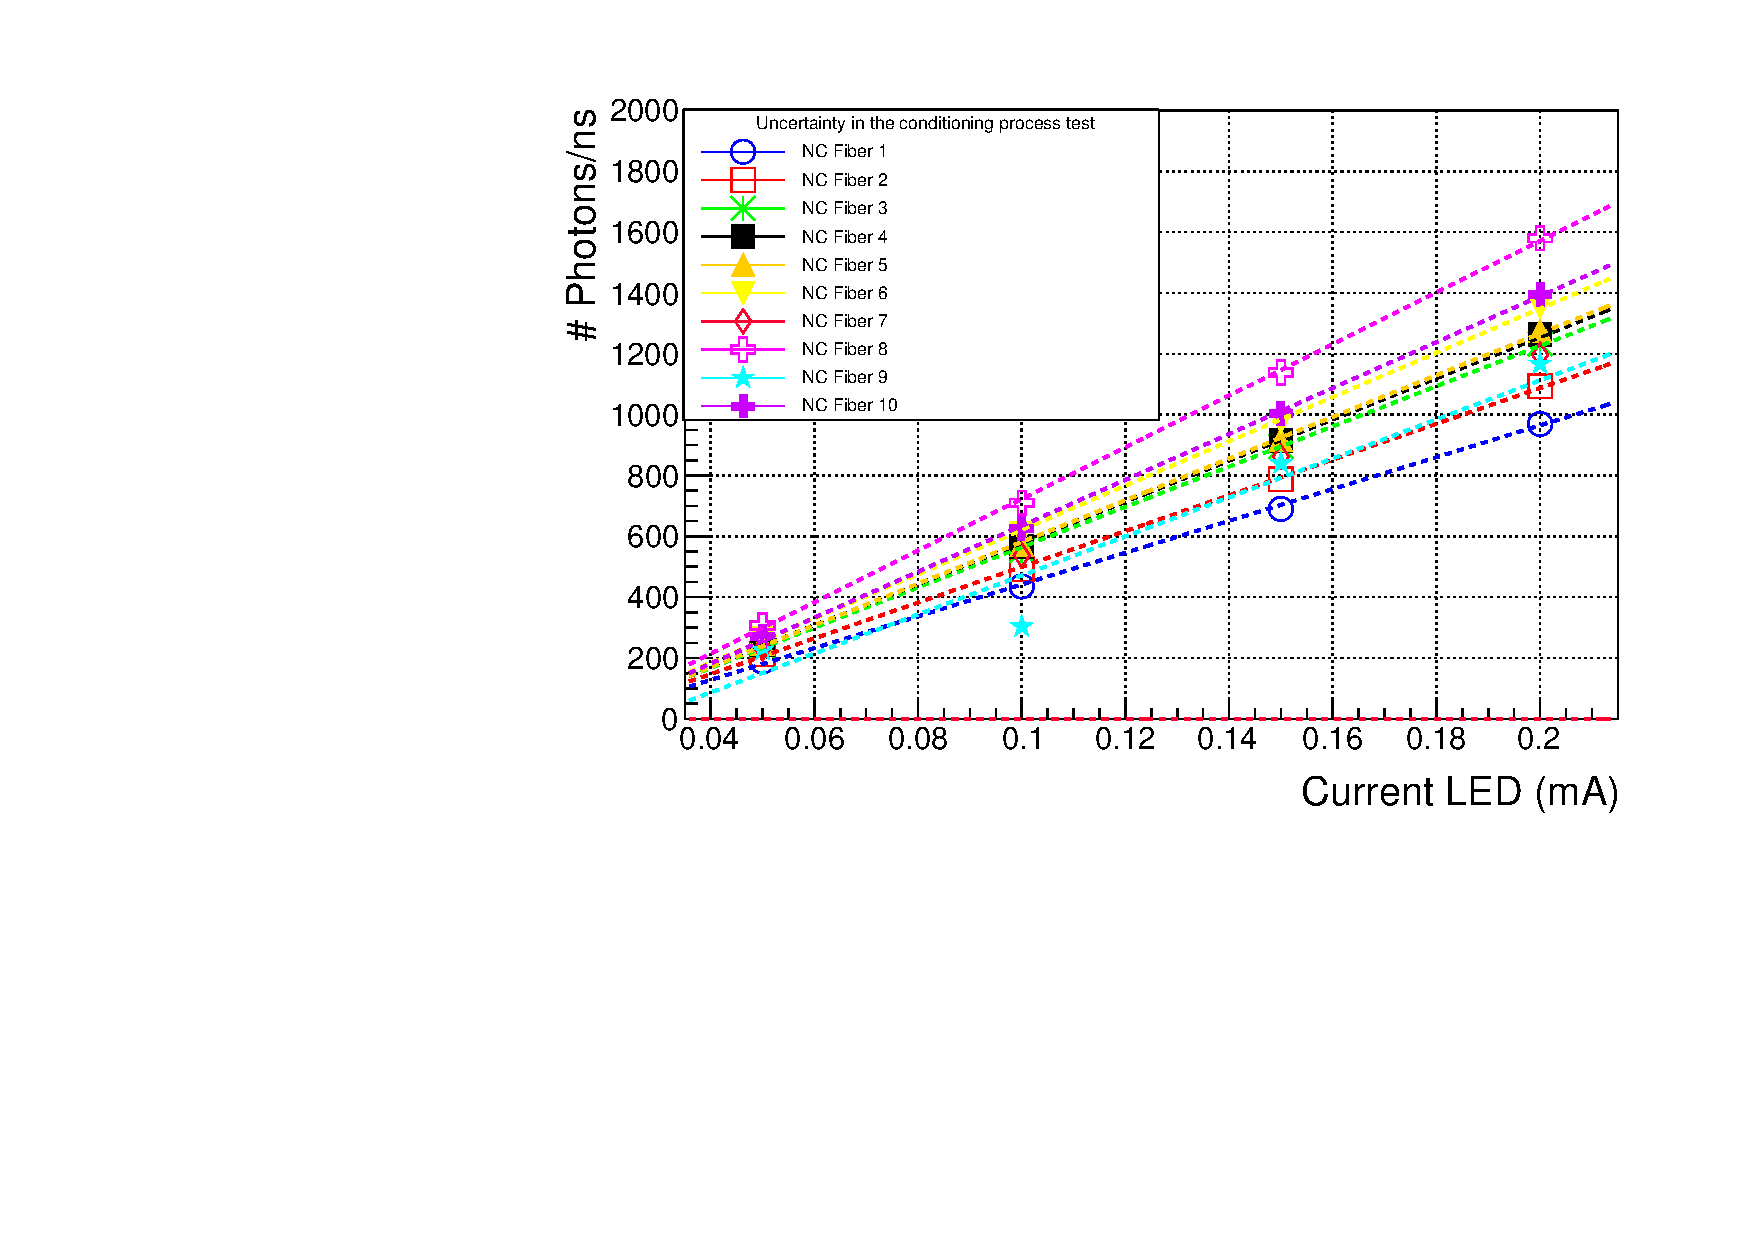
\includegraphics[scale=0.7]{4ResearchAndDevelopments/41Fibers/10_Different_samples_NoClad.pdf}
\caption{Rate of photons reaching the PMT for uncladded fibers. Error bars are smaller than the dot size.\label{fig:10samplesNC}}
\end{figure}

\begin{figure}
\centering
    %\begin{subfigure}[b]{0.6\textwidth}
    %\centering
    %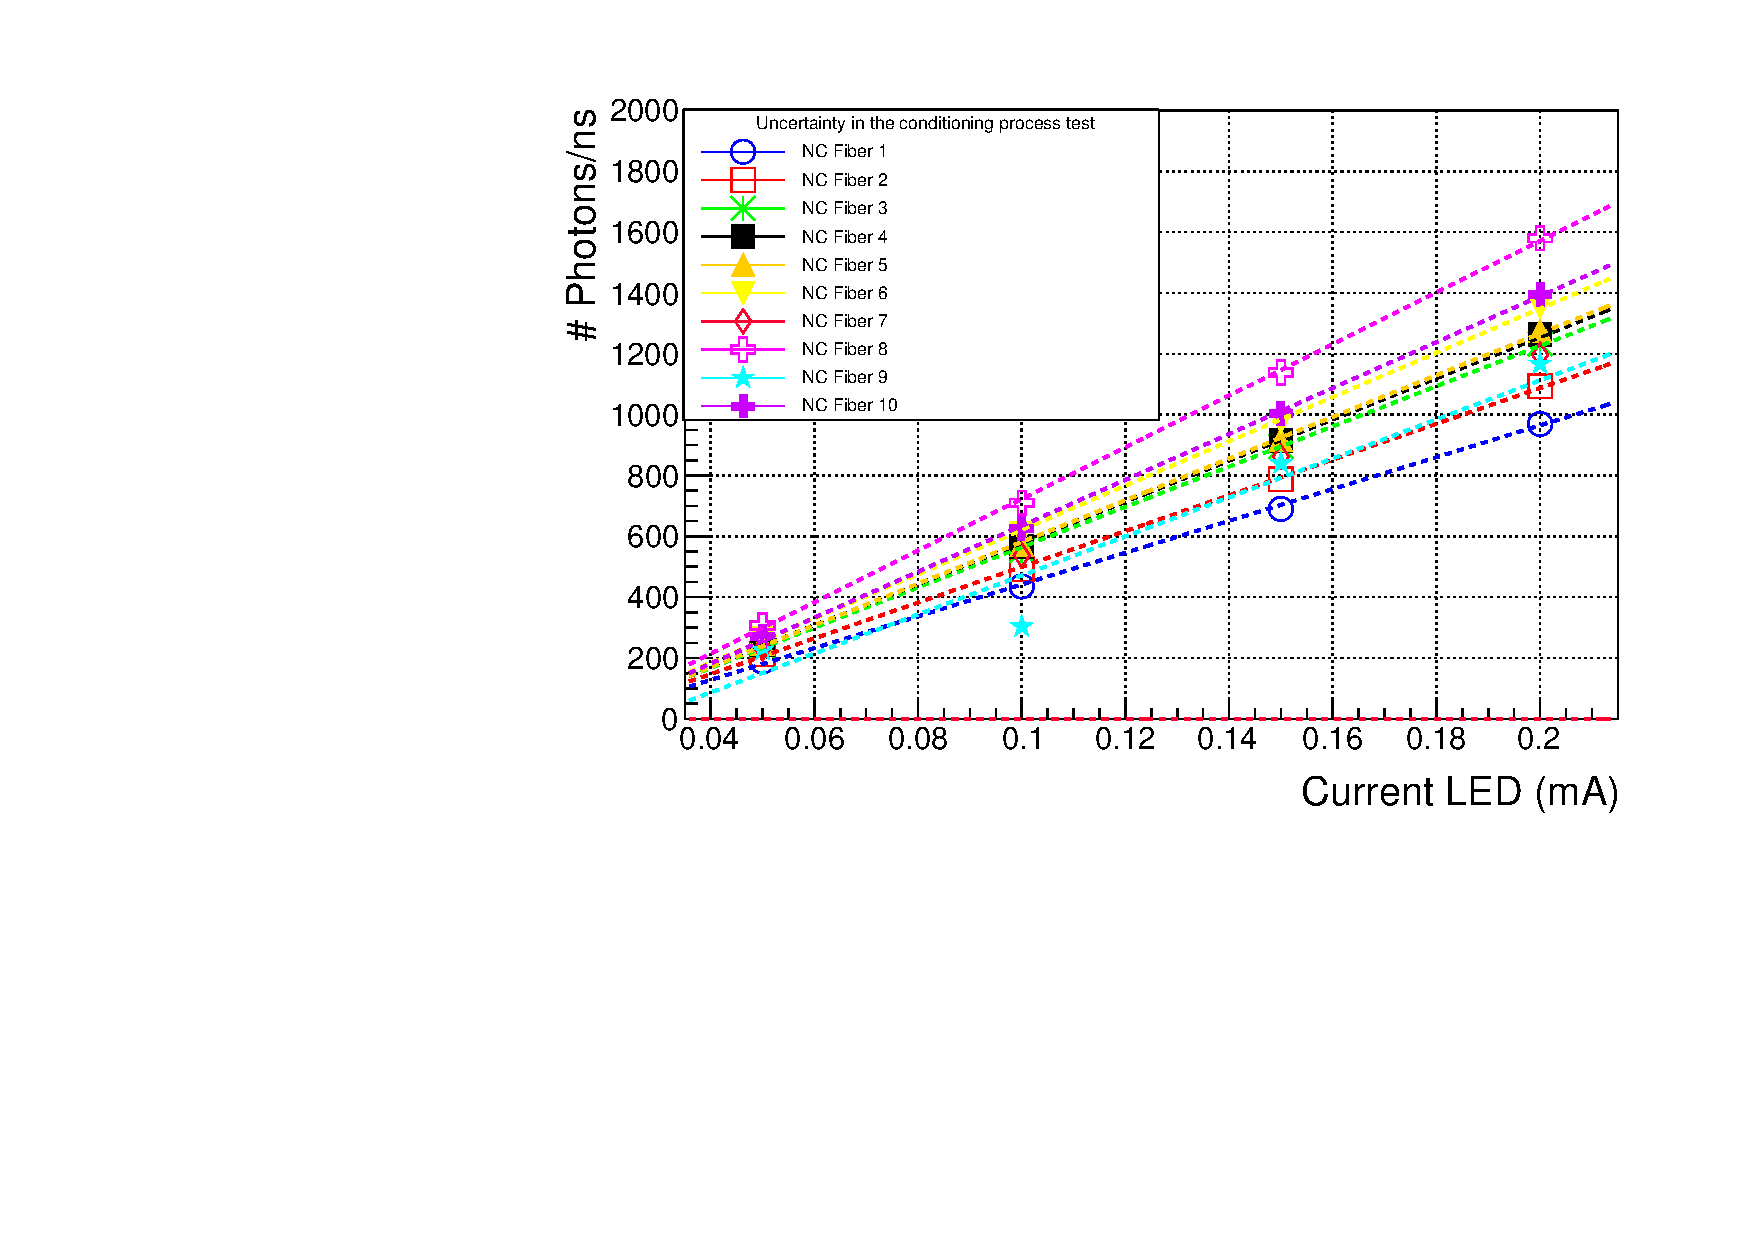
\includegraphics[width=\textwidth]{4ResearchAndDevelopments/41Fibers/10_Different_samples_NoClad.pdf}  
    %\caption{Number of photons/ns reaching the PMT for uncladded fibers.\label{subfig:10samplesNC}}
    %\end{subfigure}
    %\hfill
    \begin{subfigure}[b]{1\textwidth}
    \centering
    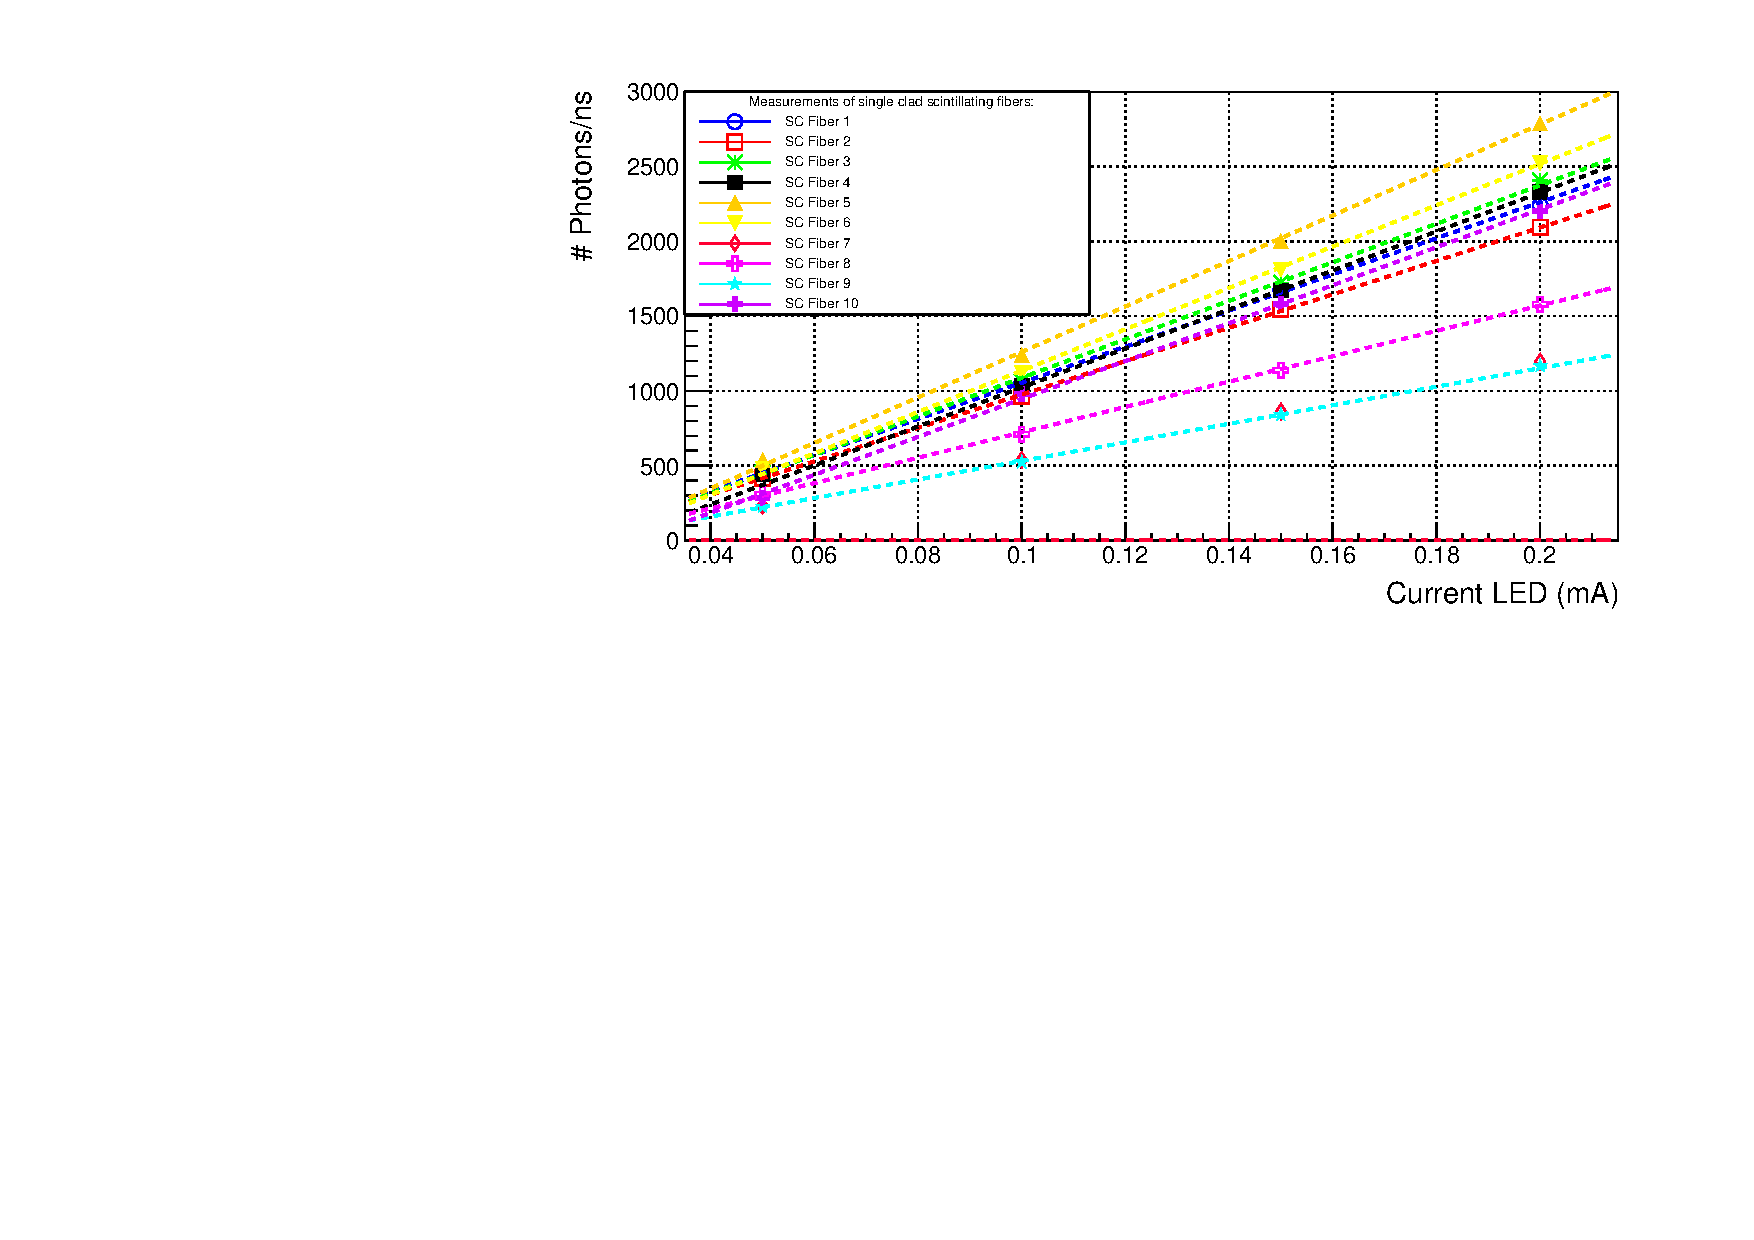
\includegraphics[width=\textwidth]{4ResearchAndDevelopments/41Fibers/10_Different_samples_SingleClad.pdf}  
    \caption{\label{subfig:10samplesSC}}
    \end{subfigure}
    \hfill
    \begin{subfigure}[b]{1\textwidth}
    \centering
    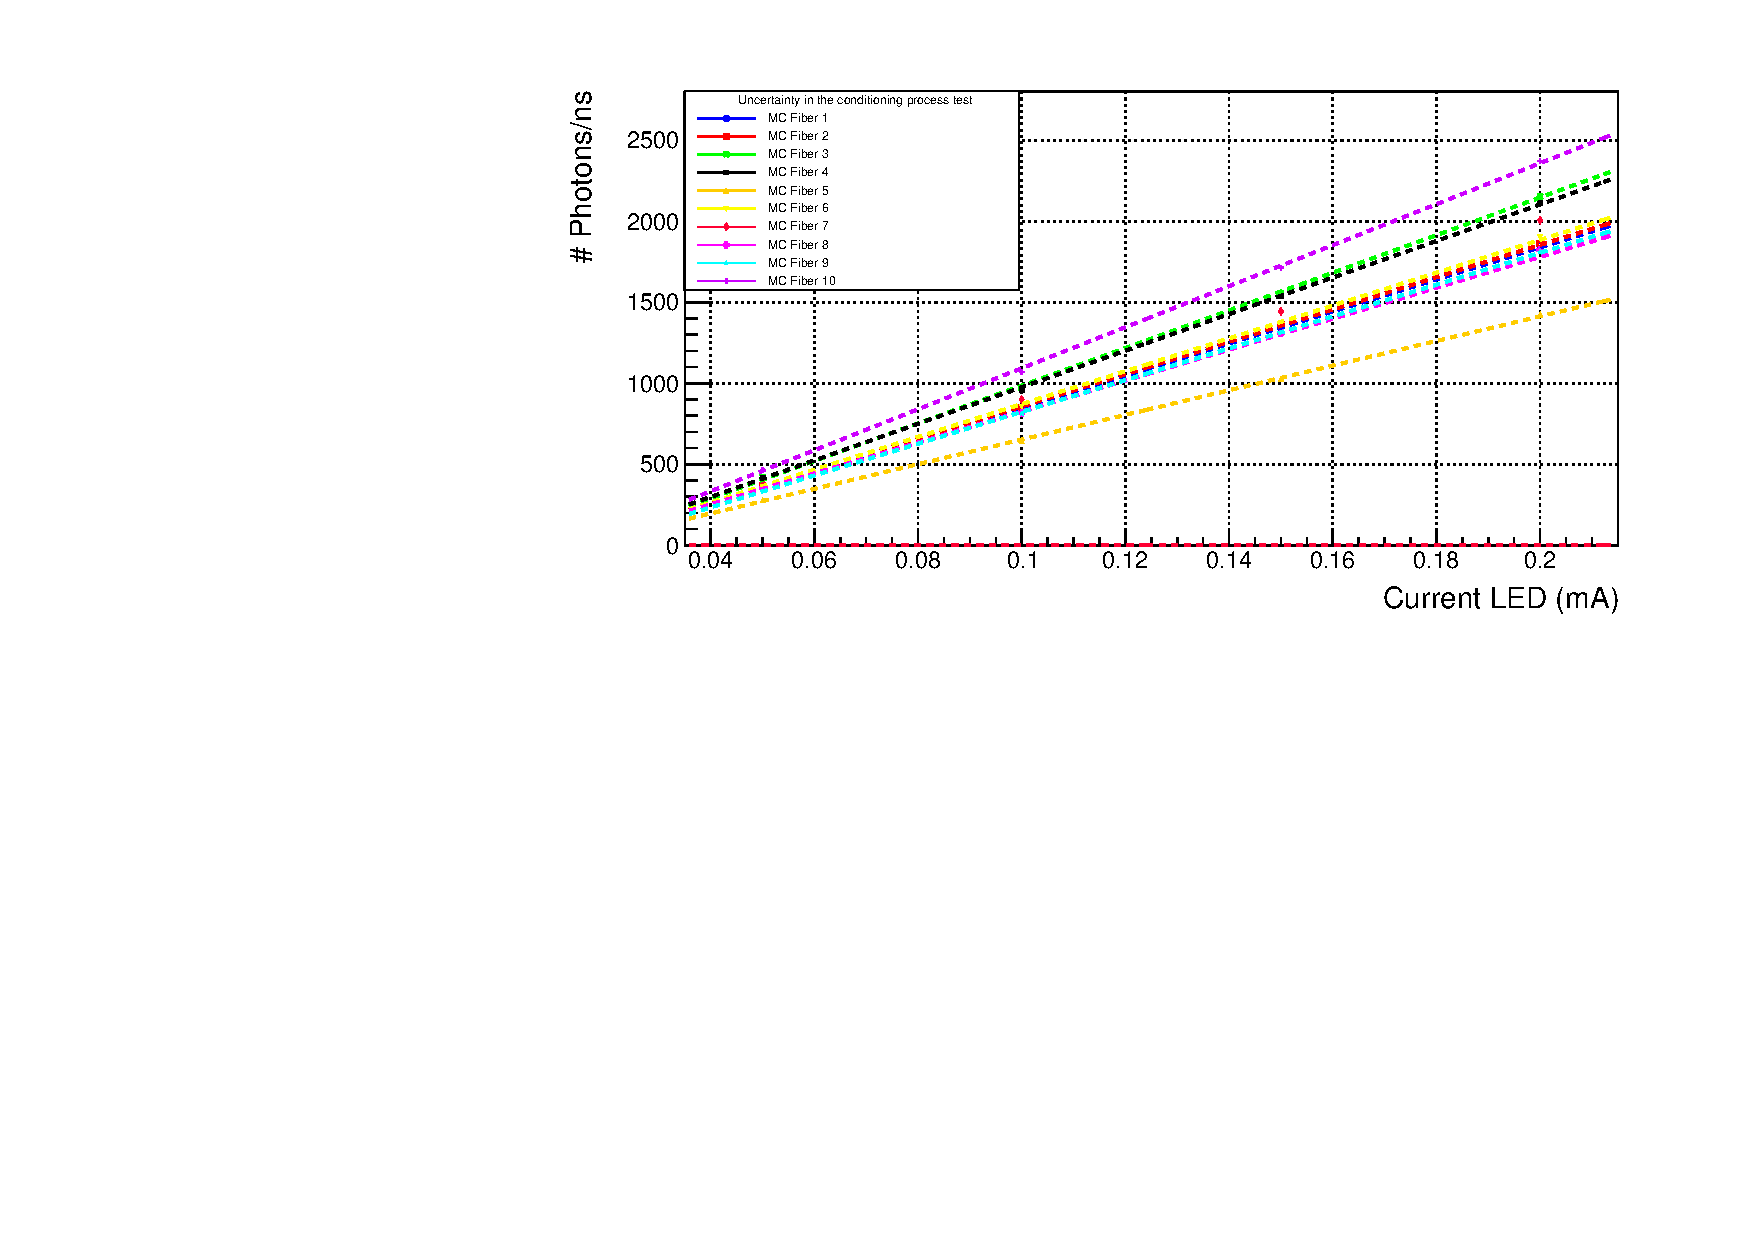
\includegraphics[width=\textwidth]{4ResearchAndDevelopments/41Fibers/10_Different_samples_MultiClad.pdf}  
    \caption{\label{subfig:10samplesMC}}
    \end{subfigure}
 \caption{Photon rate reaching the PMT for ten different fibers. a) Single clad fibers. b) Multiclad fibers. Error bars are smaller than the dot size.}
 \label{fig:10samplesThreeTypes}
\end{figure}
The average of the photon rate and the relative standard deviation versus LED intensity for each type of fiber are given in Tables \ref{tab:10DifferentSamples} and \ref{tab:RelativeStandardDeviation3FiberTypes} respectively, and are plotted in Figure \ref{fig:AveregeThreeFiberTypes}. As it can be noticed in Figures \ref{fig:10samplesNC} and \ref{fig:10samplesThreeTypes}, the fiber response is quite linear with current. Single clad and multiclad fibers give larger signals than uncladded fibers (a factor two in the case of single clad), which indicates that the clad has a significant effect on the fiber collection efficiency. It can also be observed in Table \ref{tab:RelativeStandardDeviation3FiberTypes} that the relative standard deviation $\sigma^{rel}_{sys}$ does not vary with the LED intensity. The largest uncertainty was found for single clad fibers, despite of their higher light collection. This is most probably due to the cleaving process that produces cracks in the clad, as observed in Figure \ref{fig:CleavingFiberEnd}. This damage seems to be reduced for multi-clad fibers, probably due to their larger mechanical resistance.

\begin{table}[h]
\centering{}%
\begin{tabular}{lccc}
\toprule 
Intensity (mA) & \multicolumn{3}{c}{Photon rate ($10~\nano\second^{-1}$)} \tabularnewline
\midrule
Fiber type & Uncladded & Single clad & MultiClad \tabularnewline
\midrule
\midrule 
$0.05$ & $24.5 \pm 1.1$ & $38 \pm 3$ & $37.7 \pm 1.5$ \tabularnewline
$0.1$ & $57 \pm 3$ & $92 \pm 7$ & $87 \pm 4$ \tabularnewline
$0.15$ & $92 \pm 4$ & $149 \pm 12$ & $140 \pm 6$ \tabularnewline
$0.2$ & $127 \pm 6$ & $205 \pm 17$ & $193 \pm 8$ \tabularnewline
\bottomrule
\end{tabular}
\caption{Photons rate versus LED intensity for the different type of fibers.}
\label{tab:10DifferentSamples}
\end{table}

\begin{table}[h]
\centering{}%
\begin{tabular}{lccc}
\toprule 
Intensity (mA) & \multicolumn{2}{c}{$\sigma^{rel}_{sys}(\%)$} \tabularnewline
\midrule
Fiber type & Uncladded & Single clad & MultiClad \tabularnewline
\midrule
\midrule
$0.05$ & $4.4$ & $8.7$ & $4$ \tabularnewline
$0.1$ & $4.6$ & $8$ & $4$ \tabularnewline
$0.15$ & $4.3$ & $8.1$ & $4$ \tabularnewline
$0.2$ & $4.4$ & $8.1$ & $3.9$ \tabularnewline
\midrule 
Mean & $4.4$ & $8.2$ & $4$ \tabularnewline
\bottomrule
\end{tabular}
\caption{Relative standard deviation of the photon rate $\sigma^{rel}_{sys}(\%)$ versus LED intensity for the different fiber types.}
\label{tab:RelativeStandardDeviation3FiberTypes}
\end{table}

\begin{figure}[h]
\centering
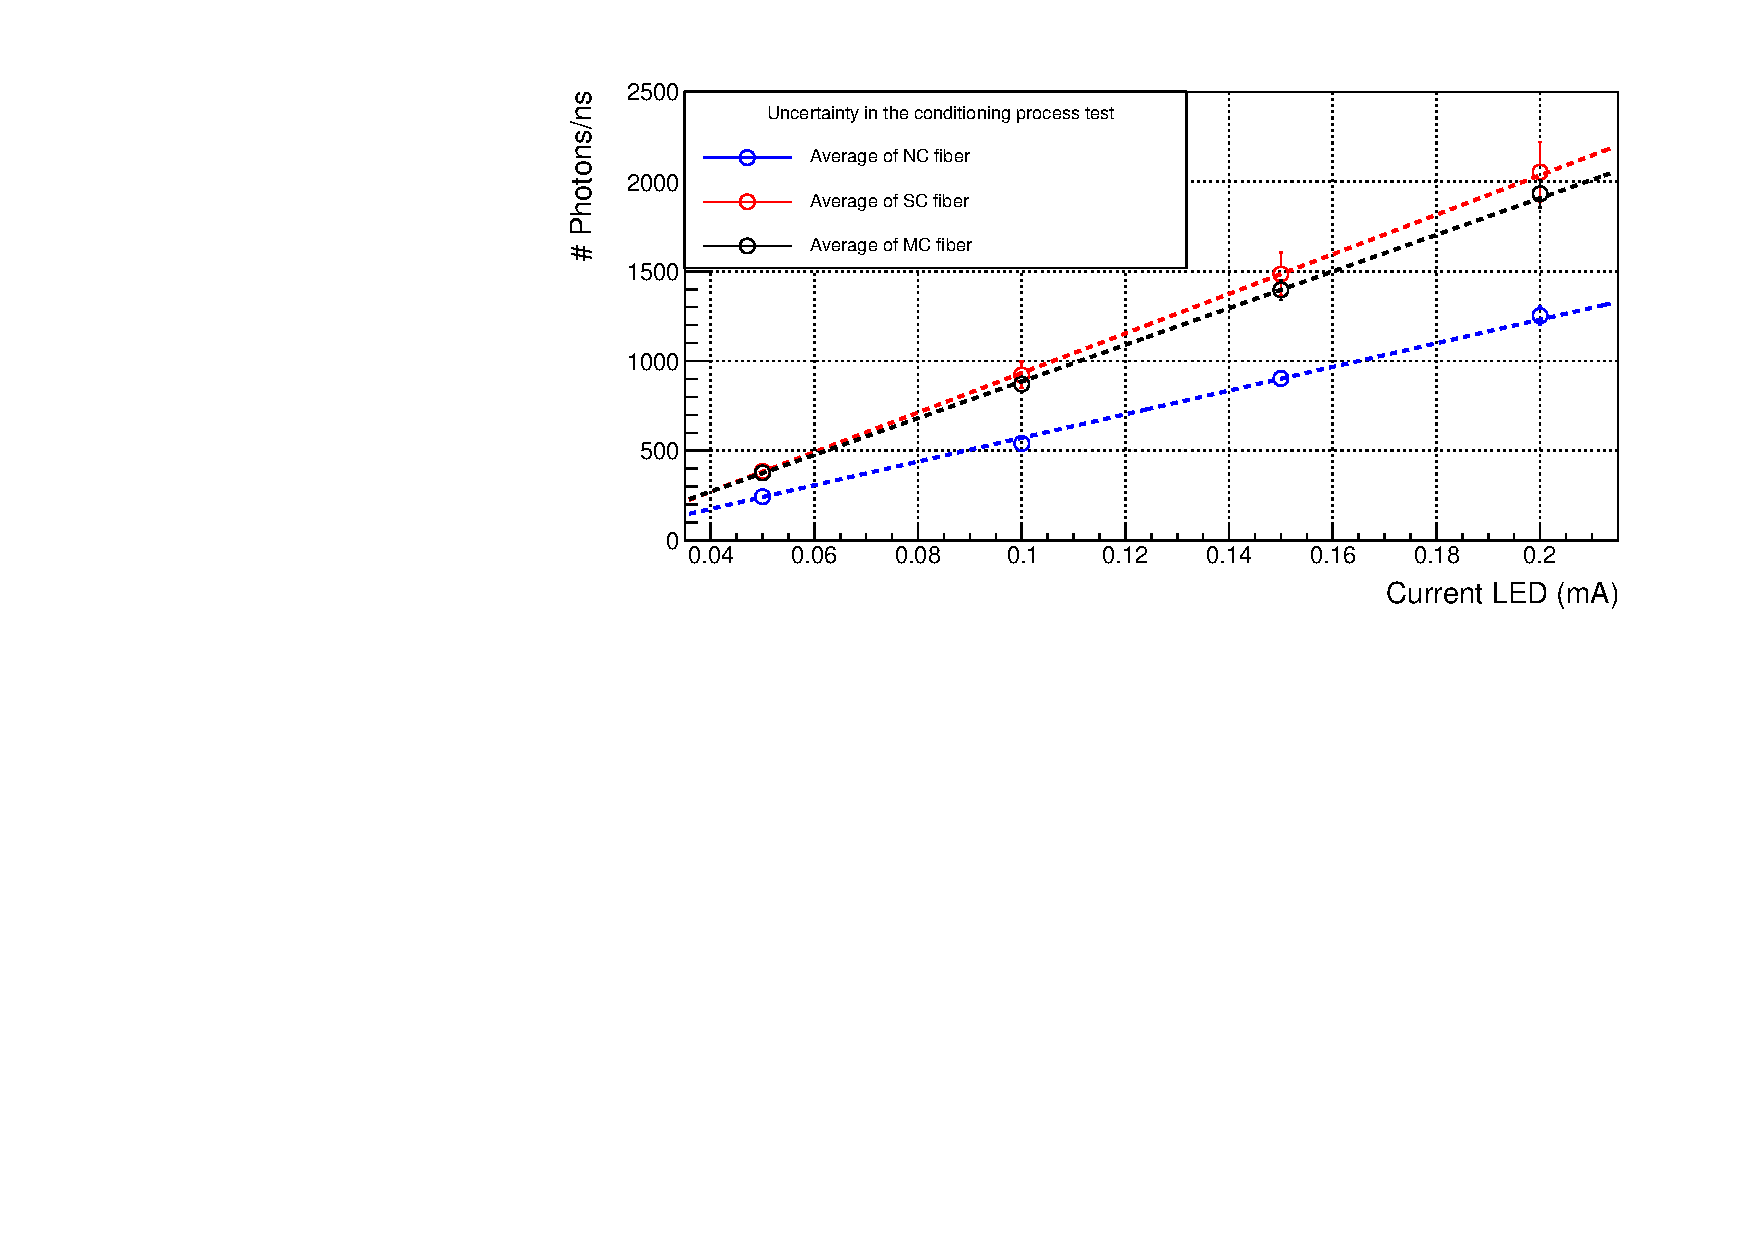
\includegraphics[scale=0.6]{4ResearchAndDevelopments/41Fibers/10_Different_Samples_Average_3_Fiber_Types.pdf}
\caption{Average photon rate versus LED current for 10 samples of different fiber types (uncladded, singleclad and multiclad fibers). Error bars are smaller than the dot size.\label{fig:AveregeThreeFiberTypes}}
\end{figure}

%The relative standard deviation are also presented in these tables, where we it can be seen that the dispersion of each fiber type for different LED intensities is practically negligible, which again verifies the correct behavior of the system. 

%There is only one point (uncladded fiber with $0.1~\milli\ampere $) that is higher than we expect. We can see in Table \ref{tab:10DifferentSamplesNoClad} that the reason for this is that its standard deviation is too high (as high as the measurement for uncladded fibers with $0.15~\milli\ampere$). The reason was found in the sample 9, whose measurement was very different from the average, incresing the standard deviation, probably due to a problem in the measurement process. We discard this sample because this result is not representative.

The average of $\sigma^{rel}_{sys}$, $\sigma^{rel}_{sys-pos}$ and $\sigma^{rel}_{sys-SF}$ are given in Table \ref{tab:RelativeStandardDeviations}. The smallest relative standard deviation was found for uncladded fibers, which means that the damage occurs mainly in the fiber clad, as illustrated in Figure \ref{fig:ResultofPolishingProcess} where cracks in the clad due to the cleaving process can be seen. It was checked under microscope that this damage only occurs at the end of the fiber. Also, the largest relative standard deviation is obtained for single clad fibers, which indicates that a second clad increases the tolerance of the fiber to conditioning.

\begin{table}[htbp]
\centering{}%
\begin{tabular}{lccc}
\toprule 
Fiber type & $\sigma^{rel}_{sys}$ (\%) & $\sigma^{rel}_{sys-pos}$ (\%) & $\sigma^{rel}_{sys-SF}$ (\%) \tabularnewline
\midrule
\midrule 
Uncladded & $4.4$ & $3.4$ & $2.9$ \tabularnewline
Single Clad & $8.2$ & $0.9$ & $8.1$ \tabularnewline
Multiclad & $4$ & $1$ & $3.8$ \tabularnewline
\bottomrule
\end{tabular}
\caption{Measured relative standard deviations $\sigma^{rel}_{sys}$, $\sigma^{rel}_{sys-pos}$ and $\sigma^{rel}_{sys-SF}$.}
\label{tab:RelativeStandardDeviations}
\end{table}

In summary, the relative statistical deviation due to fiber conditioning was quantified for the different fiber types. It was found that a fiber clad improves the photon collection efficiency but at the cost of worsening its standard deviation. Larger uncertainties (a factor two) in the light collection were observed in single clad fibers compared to multiclad and uncladded ones. This may be due to the damage in the clad produced during the cleaving process of these fibers. %Therefore, it was decided to use uncladded fibers for the TRITIUM detector. 

The absolute photon collection efficiency of $10~\cm$ scintillating fibers $CE_{10}$ was measured for each type of fiber. Ten different fibers of $10~\cm$ length for each fiber type were prepared and the photon rates were measured and summarized in Table \ref{tab:10DifferentSamplesAlltypes}. $CE_{10}$ was calculated by comparing the collected photon rate to that for a fiber length of $20~\cm$. 
\begin{equation}
CE_{10}=\frac{R_{ph}(20~\cm)}{R_{ph}(10~\cm)}=e^{-10/L}=96\%
\label{eq:CollectionEfficiency}
\end{equation}
where $L=270~\cm$ is the attenuation length provided by the manufacturer. Considering an exponential attenuation of the photon rate $N_{ph}$ with length \cite{Leo},
\begin{equation}
N_{ph}(x) = N_{ph}(x_0) \times e^{-(x-x_0)/L}
\label{eq:ExponentialAttenuation}
\end{equation}
The absolute collection efficiency obtained was somewhat smaller than the obtained from the attenuation length for all the scintillating fiber types.

\begin{table}[htbp]
\centering{}%
\begin{tabular}{lccc}
\toprule 
Intensity (mA) & \multicolumn{3}{c}{Photon rate ($10^{2}~\nano\second^{-1}$)} \tabularnewline
\midrule
Fiber type & Uncladded & Single clad & MultiClad \tabularnewline
\midrule
\midrule
$0.05$ & $3.2 \pm 0.6$ & $5.5 \pm 0.7$ & $4.8 \pm 0.8$ \tabularnewline
$0.1$ & $7.4 \pm 1.4$ & $12.7 \pm 1.6$ & $11.1 \pm 1.9$ \tabularnewline
$0.15$ & $11.8 \pm 2.3$ & $19.8 \pm 2.3$ & $18\pm 3$ \tabularnewline
$0.2$ & $16 \pm 3$ & $25.1 \pm 2.1$ & $23 \pm 4$ \tabularnewline
\bottomrule
\end{tabular}
\caption{Average photon rate versus LED intensity for 10 different samples of $10~\cm$ length for uncladded, single clad and multiclad fibers.}
\label{tab:10DifferentSamplesAlltypes}
\end{table}

%The collection efficiency  to $CE_{100}$ was calculated from $CE_{10}$ by assuming an exponential attenuation of the signal in length as follow \cite{}.

\begin{table}[htbp]
\centering{}%
\begin{tabular}{lcc}
\toprule 
Fiber type & $CE_{10}$ (\%) \tabularnewline
\midrule
\midrule 
Uncladded & $76 \pm 8$ \tabularnewline
Single clad & $78 \pm 6$ \tabularnewline
Multiclad & $83 \pm 7$ \tabularnewline
\bottomrule
\end{tabular}
\caption{Average collection efficiency $CE_{10}$ for different types of scintillating fibers.}
\label{tab:CollectionEfficiencyOfFibers}
\end{table}


%The collection efficiency, $CE_{100}$, given by the manufacturer Saint-Gobain is in the range $3.44\%-7\%$ \cite{DataSheetBCF12Fiber}. Our measurements, given in Table \ref{tab:CollectionEfficiencyOfFibers}, are close but slightly higher than the manufacturer values which could be attributed to our use of collimated photons.

%As collimated photons were used in this study, the fact that our results are in the best side is justified. As it can be seen in Table \ref{tab:CollectionEfficiencyOfFibers}, our measured values are very close to those provided by the manufacturer. %The difference between this value for the three types of fiber studied is not as large as it was expected. A possible reason is that the difference in fiber length is only $10~\cm$ and it may not be enough to see this effect. It could be interesting to repeat these tests with a larger difference in fiber length.